HPC simulations create large amounts of data that are then read offline by analysis tools. 
In the following we present the traditional approaches to parallel I/O as well
as the problems they pose in terms of performance variability. We then dive into the trend toward
coupling simulations with analysis and visualization tools, going from offline to in situ analysis and
visualization.

\subsection{I/O and Storage for Large-Scale HPC Simulations}
			
			Two I/O approaches are commonly have been traditionally used for performing I/O in large-scale simulations.
%
			\begin{description}
		
			\item[The File-per-process] approach consists of having each process access its own file.
			This reduces possible interference between the I/O of different processes, but  increases the number of metadata operations. 
			This is especially a problem for file systems with a single metadata server, such as Lustre~\cite{schwan2003lustre}. 
			It is also hard to manage the large number of files thus created and have them read by  analysis or visualization 
			codes that use a different number of processes
			
			\item[Collective I/O] leverages communication phases between
			processes to aggregate access requests and reorganize them. These operations
			are typically used when several processes need to access different parts
			of a shared file, and benefit from tight interactions between the file system
			and the MPI-I/O layer in order to optimize the application's access pattern~\cite{prost2006mpi}.
			
			\end{description}
%
			\subsubsection{Variability in Traditional I/O Approaches}

			The periodic nature of scientific simulations, which alternate between computation and I/O phases,
			leads to burst of I/O activity. The overlap between computation and I/O is reduced, so that both the compute 
			nodes and the I/O subsystem may be idle for periods of time.
		
			With larger machines, the higher degree of I/O concurrency between processes of a single application
			or between concurrent applications pushes the I/O system to its limits. This
			leads to a substantial variability in I/O performance.
			Reducing or hiding this variability is critical, as it is an effective way to make
			a more efficient use of these new computing platforms through improved
			predictability of the behavior and of the execution time of applications.
			
			Figure~\ref{fig:ior:variability} illustrates this variability with the IOR application~\cite{shan2007using},
			a typical benchmark used to evaluate the performance of parallel file systems with pre-defined
			I/O patterns. It shows that even with very well optimized I/O (each process here writes the same amount
			of data contiguously in a separate file using large requests that match the file system's distribution policy) 
			there is a large difference in the time taken by each
			process to complete its I/O operations within a single I/O phase and also across I/O phases.
			Since during these I/O phases all processes have to wait for the slowest one before resuming computation, 
			this I/O variability leads to a waste of performance and to unpredictable overall run times.
			I/O variability is therefore a key issue that we aim to address in this paper.
			
			\begin{figure}
				\begin{center}
				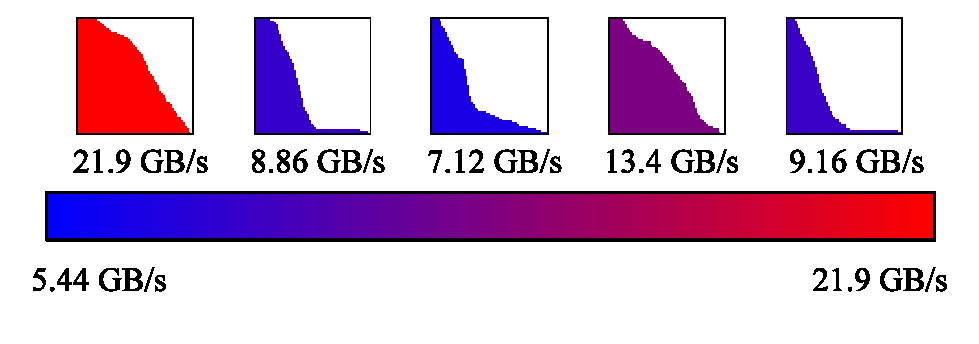
\includegraphics[width=10cm]{figures/variability.eps}
				\caption[somthing]{Variability across processes and across I/O phases in the IOR benchmark using a file-per-process approach
				on Grid'5000's Rennes site~\protect\cite{grid5000}, with a PVFS2~\protect\cite{carns2000pvfs} file system.
				Each graph represents a write phase. The 576 processes are sorted by write time on the $y$ axis and
				an horizontal line is draw with a length proportional to this write time. These graphs are normalized
				so that the longest write time spawns the entire graph. Each graph is colored according to
				a scale that gives the aggregate throughput of the phase, that is, the total amount
				of data written divided by the write time of the slowest process.\footnotemark}\label{fig:ior:variability}
				\end{center}
			\end{figure}
			
			\AtBeginShipoutNext{\footnotetext{Due to the use of colors, this figure may not be properly interpretable if this document
			was printed in black and white. Please refer to an electronic version.}}
			
		\subsubsection{Causes and Effects of the I/O Variability}
		
			Skinner at al.~\cite{skinner2005understanding} point out four causes of 
			performance variability in supercomputers (here presented in a different order).
%
			\begin{enumerate}
			
			\item Communication, causing synchronization between
			processes that run within the same node or on separate nodes. In
			particular, network access contention causes collective
			algorithms to suffer from variability in point-to-point communications.
			
			\item Kernel process scheduling, together with the jitter introduced by
			the operating system.
			
			\item Resource contention within multicore nodes, caused by
			several cores accessing shared caches, main memory and network devices.
			
			\item Cross-application contention, which constitutes a random
			variability coming from simultaneous accesses to shared components of the
			computing platform, such as the network or the storage system, by distinct applications.
		
			\end{enumerate}
%
			Future systems will have additional sources of variability, such as power management, and fault masking activities.
			Issues 1 and 2, respectively, cause communication and computation jitter.
			Issue 1 can be addressed through more efficient network hardware 
			and collective communication algorithms. The use of 
			lightweight kernels with less support for process scheduling can alleviate issue 2. 
			Issues 3 and 4, on the other hand, cause I/O performance variability.
		
			At the level of a node, the increasing number of cores per node in recent machines makes 
			it difficult for all cores to access the network all at once with an optimal 
			throughput. Requests are serialized in network devices, leading to a different service
			time for each core. This problem is further amplified by the fact that an I/O 
			phase consists of many requests that are thus serialized in an unpredictable manner.

			Parallel file systems also represent a well-known bottleneck and a source of high
			variability~\cite{uselton2010parallel}. The time taken
			by a process to write some data can vary by several orders of
			magnitude from one process to another and from one I/O phase to
			another depending on many factors, including (1) network contention 
			when several nodes send requests to the same I/O server~\cite{dorier2014calciom}, 
			(2) access contention at the level of the file system's metadata server(s) 
			when many files are created simultaneously~\cite{dorier:inria-00614597},
			(3) unpredictable parallelization of I/O requests across I/O servers due to different 
			I/O patterns~\cite{lofstead2010managing}, (4) additional disk-head movements due 
			to the interleaving of requests coming from different processes or applications~\cite{gainaru2014scheduling}.
			Other source of I/O variability at disk level include the overheads of RAID group reconstruction, 
			data scrubbing overheads, or various firmware activities.
		
			Lofstead et al.~\cite{lofstead2010managing} present I/O variability in terms
			of \emph{interference}, with the distinction between \emph{internal
			interference} caused by access contention between processes of
			the same application, and \emph{external interference} that are due to
			sharing the access to the file system with other applications,
			possibly running on different clusters.
			While the sources of I/O performance variability are numerous and difficult to track, we can indeed
			observe that some of them originate from contentions within a single application,
			while other come from the contention between multiple applications concurrently running on
			the same platform. The following section describes how to tackle these two sources of contention.
						
		\subsubsection{Approaches to Mitigate the I/O Variability}

			While most efforts today address performance and scalability issues for
			specific types of workloads and software or hardware components, few
			efforts target the causes of performance variability. We highlight two
			practical ways of hiding or mitigating the I/O variability.

			\paragraph{Asynchronous I/O}
				The main solution to prevent an application from being impacted by its I/O consists
				of using asynchronous I/O operations, i.e., non-blocking operations that proceed in
				the background of the computation.
	
				The MPI 2 standard proposes rudimentary asynchronous I/O functions
				that aim to overlap computation with I/O. Yet these functions are available only 
				for independent I/O operations. Besides, popular implementations of the MPI-I/O
				standard such as ROMIO~\cite{thakur1999on} actually implement most of these functions
				as synchronous. Only the small set of functions that handle contiguous accesses have
				been made asynchronous, provided that the backend file system supports it.
	
				Released in 2012, the MPI 3 standard completes this interface with asynchronous 
				collective I/O primitives. Again, their actual implementation is mostly synchronous.
				As of today, there is no way to leverage completely asynchronous I/O using only MPI-I/O.
				Higher-level libraries such as HDF5~\cite{hdf5,folk1999hdf5} or NetCDF \cite{netcdf} 
				have also no support yet for asynchronous I/O.
			
			\paragraph{Dedicated I/O Resources}
				Over the past few years, dedicated I/O resources have been proposed to address the
				limitation of MPI implementations in terms of asynchronous I/O. These resources can take various forms. 
				Explicit I/O threads~\cite{fu2012iothreads} have been used to achieve fully asynchronous
				I/O at the potential price of additional OS jitter.
				Dedicated cores have been proposed to leverage a subset of cores in each multicore node used 
				by the application~\cite{dorier2012damaris,li2010functional}, and have them perform I/O operations on behalf of the
				cores that run the application. Staging areas~\cite{abbasi2009datastager,nisar2009scaling,prabhakar2011provisioning} is another
				approach that usually consists of dedicated nodes deployed along with an application.
				Forwarding nodes~\cite{ali2009scalable,stone2006pdio} and burst buffers~\cite{liu2012role,ma2006highlevel} consist of a set 
				of nodes, independent of the applications and interposed between the compute nodes 
				and the storage system. These nodes may feature a larger memory capacity than compute nodes,
				in the form of SSDs or NVRAMs.
				
				This trend toward using dedicated resources has benefited the field of data
				analysis and visualization as well, where dedicated cores or nodes are seen as new ways to 
				efficiently get access to simulations' data as they are generated. The next section
				explores this trend in more details.
				
\subsection{Analysis and Visualization: an Overlooked Process}

	Data produced by HPC simulations can serve several purposes. 
	One of them is fault tolerance using a checkpoint/restart method.
	The other, and most important, is the analysis and visualization of the simulated phenomenon.
	Analysis and visualization are important components of the process that leads
	from running a simulation to actually \emph{discovering knowledge}.
	
	Given the increasing computation power in recent machines and the trend toward using dedicated resources,
	it will become more and more common to couple the simulation with the analysis and visualization tools.
	Simulation/Visualization coupling consists of making the simulation send its data directly to
	a visualization software instead of storing it and processing it offline.
	This approach, termed \textit{in situ visualization} and illustrated in
	Figure~\ref{fig:simviz} (b), has the advantage of bypassing the 
	storage system and producing results faster. It also allows scientists to control their simulations
	as they run, efficiently overlapping simulation and knowledge discovery.
	
	\begin{figure}
		\begin{center}
		\subfigure[Traditional Scientific Workflow]{
			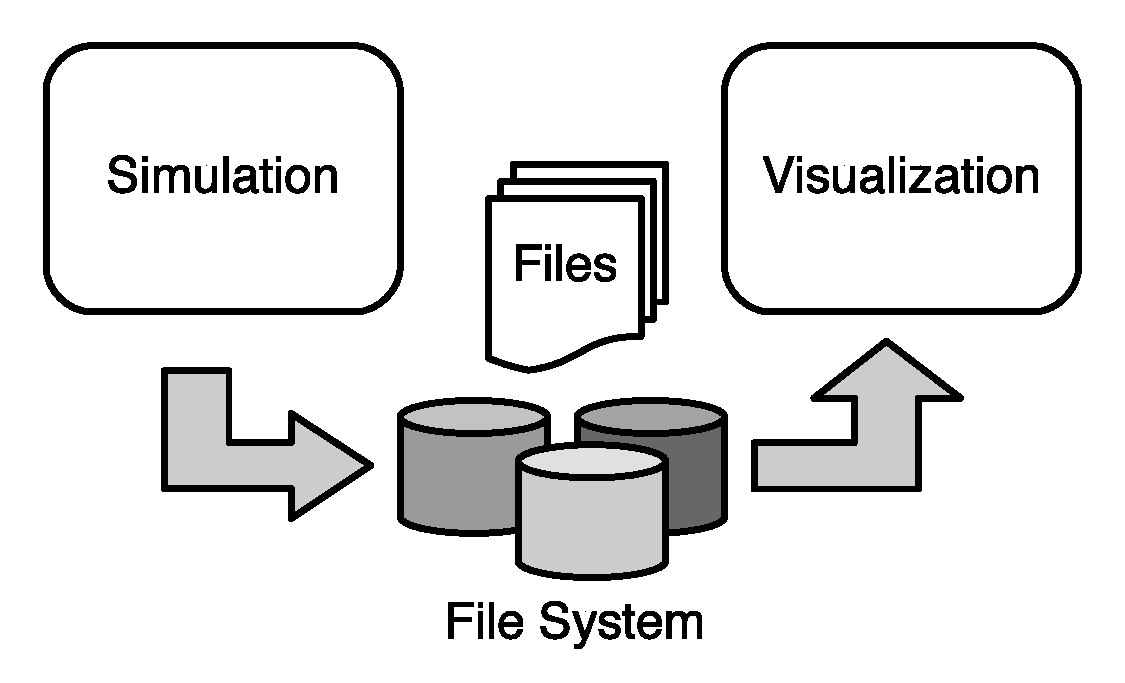
\includegraphics[width=5.5cm]{figures/simviz1.eps}
		}
		\subfigure[Coupling Simulation/Visualization]{
			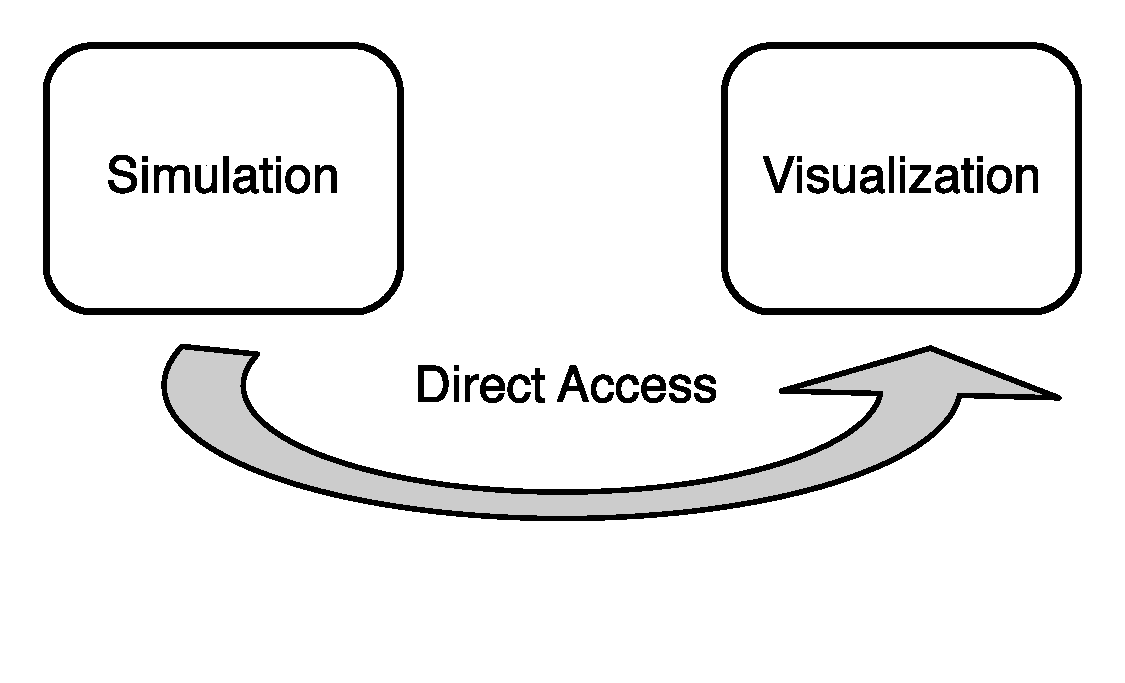
\includegraphics[width=5.5cm]{figures/simviz2.eps}
		}
		\caption{Two approaches to retrieve 
		insight from large-scale simulations: (a) the traditional approach of storing data in a parallel
		file system and reading it offline, (b) the new trend towards simulation/visualization coupling.}\label{fig:simviz}
		\end{center}
	\end{figure}
	
	\subsubsection{A Taxonomy of In Situ Visualization Methods}

	Several in situ visualization strategies exist that we separate into two main categories 
	--tightly coupled and loosely coupled-- depending on where visualization tasks run.

		\paragraph{Tightly-Coupled In Situ Visualization} 
		In a tightly-coupled scenario, the analysis and visualization codes run on the same node 
		as the simulation and share its resources. The main advantage of this scenario is the proximity 
		to the data, which can be retrieved directly from the memory of the simulation. 
		Its drawback lies in the impact that such analysis and visualization tasks can have on the performance 
		of the simulation and on the variability of its run time. Within this category, we make a distinction between
		\emph{time partitioning} and \emph{space partitioning}. 
		
		Time-partitioning visualization consists of periodically stopping the simulation to perform visualization tasks. 
		This is the most commonly used method. For example, it is implemented in VisIt's \emph{libsim}
		library~\cite{whitlock2011parallel} and ParaView's \emph{Catalyst} 
		library~\cite{fabian2011paraview,catalyst}.

		In a space-partitioning mode, dedicated cores perform visualization in parallel with the simulation.
		This mode poses challenges in efficiently sharing data between the cores running the simulation and
		the cores running the visualization tasks, as these tasks progress in parallel. It also
		reduces the number of cores available to the simulation.
		
		\paragraph{Loosely-Coupled In Situ Visualization} 
		In a loosely coupled scenario, analysis and visualization codes run on a separate set of
		resources, that is, a separate set of nodes located either in the same supercomputer as
		the simulation~\cite{zheng2010predata,rasquin2011electronic}, 
		or in a remote cluster~\cite{malakar2010adaptive}. 
		The data is sent from the simulation to the visualization nodes through the network. 
		
		Some in situ visualization frameworks such as GLEAN~\cite{hereld2011toward} can be considered hybrid, placing
		some tasks close to the simulation in a time-partitioning manner while other tasks
		run on dedicated nodes.
	
	\subsubsection{From Offline to In Situ Visualization: Another Source of Variability}
	
		The increasing amounts of data generated by scientific simulations also leads to performance
		degradations when it comes to reading back data for analysis and visualization~\cite{childs2010extreme,yu2005study}.
		While I/O introduces run time variability, in situ analysis and visualization can also negatively impact
		the performance of the simulation/visualization complete workflow. 
		For instance, periodically stopping the simulation to perform in situ visualization in a time-partitioning manner
		leads to a loss of performance and an increase of run-time variability. 
		Contrary to the performance of the simulation itself,
		the performance of visualization tasks may depend on the
		content of the data and is therefore unbalanced across processes and across iterations.
		This variability is further amplified if the in situ visualization framework is interactive, in which case the user
		himself impacts the performance of his application.
	
		In a loosely-coupled approach to in situ visualization, sending data through the network potentially impacts the performance of
		the simulation and forces a reduced number of nodes to sustain the input of a large amount of data.
		Transferring such large amounts of data through the network also have a potentially larger
		impact on the simulation than running visualization tasks in a tightly-coupled manner.
		
\subsection{Our Vision: Using Dedicated Cores for I/O and In Situ Visualization}
	
		Despite the limitations of the traditional, offline approach to data analysis and visualization,
		users  are still seldom moving to purely in situ visualization and analysis~\cite{yu2010insitu,ma2007insitu,ma2009insitu}.
		The first reason is the development cost of such a step in large codes that were maintained for decades.
		The second reason is that storage I/O is still required for checkpoint-based fault tolerance, which makes
		offline analysis of checkpoints the natural candidate for scientific discovery.
			
		To push further the adoption of in situ visualization and increase the productivity of the overall
		scientific workflow, \emph{we postulate that a framework should be provided that deals with
		all aspects of Big Data management in HPC simulations}, including efficient I/O but also
		in situ processing, analysis and visualization of the produced data.
		Such a framework can at the same time provide efficient storage I/O for data that need to be stored,
		and efficient in situ visualization to speed up knowledge discovery and enable simulation monitoring.
		
	%	We postulate that four main requirements will drive the adoption of such a framework.
	%
	%	\begin{description}
		
	%		\item[Low impact on run time:] As explained earlier, using computational resources collocated
	%		with the simulation can affect the performance of the underlying simulation. This is 
	%		especially true when interactive systems directly connect users to their running simulation.
	%		
	%		\item[Optimized resource utilization:] Collocated simulations and
	%		post-processing codes share resources such as local memory and network bandwidth.
	%		Efficiently using these resources is critical for an approach to be suitable at a very large scale.
			
	%		\item[Low impact on the code:] Users are less likely to adopt a new
	%		approach to data management if it requires many code changes in their simulation and the 
	%		understanding of new tools~\cite{thompson2009design}, or if a I/O and visualization
	%		specialist should be consulted for that.
			
	%		\item[High adaptability:] The framework should be adaptable to many simulations and
	%		many data processing scenarios. In particular it should enable to switch visualization
	%		backends or seamlessly leverage a wide range of external data-processing libraries.
		
	%	\end{description}
	%
		Over the past 4 years we have been addressing this challenge by proposing, designing and
		implementing the Damaris system to data management.
		%, within the context of the Joint INRIA-UIUC-ANL
		%Laboratory for Petascale Computing (JLPC). 
		Damaris proposes to dedicate cores
		in multicore nodes for any type of data management task, including I/O and in situ visualization.
		We tried to make Damaris \emph{simple to use}, \emph{flexible}, \emph{portable} and \emph{efficient} 
		in order to ease its adoption by the HPC community. 
		%As a consequence, Damaris was one of the first results of the JLPC to be formally
		%validated for use on the Blue Waters Petascale project~\cite{sisneros2013application}.
		The following section gives an overview of this approach and its implementation.
		
